\chapter{Generating Encounters}
\label{chapter04}

There are many possible attributes that can be generated. We could change the size of each team,
the number of abilities of each mage, starting positions of the map, or even change the positions of the walls.

\section{Reducing the Scope of the Problem}

We chose to reduce the scope by creating a small fixed map on which all encounters will be played and balanced.
We also fix the team size of both teams to 2 mages, and each mage to 2 abilities. While this significantly reduces
the possibilities to achieve balance, there are still a lot of parameters that can be tweaked, as described in the next section.

We also put lower and upper bounds on most of the numeric values of attributes of mages and their abilities. See attached programmer documentation in the \autoref{chap:prog-doc} for more details about how attributes are represented.

\section{Approach}

We approach generating encounters as a search based problems with two different
approaches, Simulated Annealing \citep{ai-modern} and Evolution Strategies
\citep{evolution-strategies}.

To make the search algorithms as general as possible, we serialize our internal game representation into a single vector of normalized floating point values (called DNA, see \autoref{dna-format}). The algorithm then does not need to understand our game mechanics and restrictions and simply treats the DNA as a vector of floating point values.

In the case of our experiments, we chose to stick with 2v2 games on a fixed map,
where each mage has only two abilities. This was chosen both with respect to our
questionnaire, and running time of the algorithms. Choosing a larger team setup or
a bigger map (or many different maps) would be difficult for the participants,
and would also take much longer to compute our experimental data.

Taking these restrictions into mind, the DNA would then take up $96$ floating point values,
specifically: $$2 \text{ Teams} \times 2 \text{ Mages} \times ( HP + AP + 2 \times \text{AbilitySize}) = 96$$ since $\text{Ability Size} = 11$ as we need to serialize damage, cost, range, cooldown,
debuff (HP damage, AP damage, lifetime), and AOE (debuff + lifetime).

\section{Simulated Annealing}

Our initial implementation of generating the encounters was using Simulated Annealing \citep{ai-modern}. Simulated annealing works similar to a hill climbing algorithm, except that instead of always picking the best neighbor, we use a probability distribution. Neighbors with better fitness have a higher probability, but we might still take a path downhill. The amount of randomness is controlled by an external variable called temperature (or energy). As the algorithm progresses, the temperature is slowly reduced and thus allows it to converge. The main advantage over hill climbing is that simulated annealing does not immediately get stuck in a local optima, as there is always a chance it will move to a state with lower fitness value. In contrast, a hill climbing algorithm \citep{ai-modern} would always pick a neighbor with a better fitness value.

However, we had difficulty getting good results and the algorithm almost never converged. As a result, we ran an experiment to sample the search space at roughly 20 million different points, and measured the change in fitness in the neighborhood of each point. We found that in each point's neighborhood, there are roughly 5 times more points that have worse fitness than the ones that are an improvement over the current point. We also found that most of these downward changes were much steeper between 4--7x than the improving points. Our suspicion is that this is the main cause of failure of Simulated Annealing, which simply fails to find the upward slope.

\section{Evolution Strategies}

For this reason we chose to try another approach, specificially Evolution
Strategies (ES) \citep{evolution-strategies}. ES works by taking a random sample of the
neighbourhood of the current value, evaluating the fitness of each of the neighbours, and
moving to a state that is the weighted average of the neighbours with respect to their fitness.
This process is iterated until a state with suitable fitness value is found. In our experiments
we have found this approach to consistently converge much faster than simulated annealing.

ES also yields itself to easy parallelization, especially if the evaluation of the fitness
function is complicated. Since all of the neighbouring samples are completely independent,
they can be evaluated completely in parallel.

Specifically, we sample by choosing from a uniform distribution from the range $[0.75;1.25]$ (determined by the \verb|MutationDelta| constant, see \autoref{cmd-args}) and take that as a percentage update to one value in the DNA vector at a random index. We repeat this process with a probability of $p = 0.35$ (determined by the \verb|SecondMutationProb| constant). Overall, we sample $40$ neighbours this way during each iteration of ES (determined by \verb|TeamsPerGeneration| constant).

\section{Choice of the Fitness Function}

In order to evaluate the balance of a matchup, we evaluated the following three
criteria:

\begin{description}
\item [Balance] Unsurprisingly, part of the fitness function is comparing the
  strength of both teams against each other.  We consider games that end in a
    draw balanced.  If the game doesn't end in a draw, we measure the remaining
    HP percentage of the winner, and the lower it is, the more balanced the
    game was.
\item [Game length] We also put an interval restriction on game length. Ideally
  we'd want the game to last at least 2 rounds.
\item [Team difference] Lastly, since we don't to create balance by making both
  teams identical, we added a third criteria that measures the difference of
    both teams.
\end{description}

The combined fitness function is calculated as the average of the three. See \hyperref[fig:converging-es]{Figure 4.1} for an example plot of how the fitness function converges using Evolution Strategies. It is worth noting here that evaluating the fitness function (the \emph{Balance} part specifically) is computationally intensive, as it requires the whole game to be played out till the end. We also do this evaluation using an ensemble average of multiple different AIs. Specifically, we use both the Rule based AI and MCTS in the \emph{Balance} playout and take their average. This helps assure that the game is balanced despite multiple playstyles, as both the Rule based AI and MCTS play differently (see \hyperref[tab:winrates]{Table 5.1} for their comparison). You can see how the fitness function converges in \autoref{fig:converging-es}.

The combined formula is $\frac{(1 - H) + L + D}{3}$ where $H$ is the percentage of total health left at the end of the game, and

\[
L = \begin{cases}
f(\text{length} | 10, 3) &\quad\text{if length} < 20 \\
f(40 - \text{length} | 10, 2) &\quad\text{otherwise}
\end{cases}
\]

where $f$ is the cumulative distribution function for the normal distribution (see \autoref{fig:game-length}). Lastly, $D = \frac{1}{1 + \text{exp}(-60R + 1.5)}$ where $R$ is the euclidean distance between the two teams (normalized to $[0;1]$, see \autoref{fig:team-distance}). Note that the constants the above mentioned formulas were chosen by hand as to fit the game design goals (minimum game length, etc.).

\begin{figure}
	\centering
	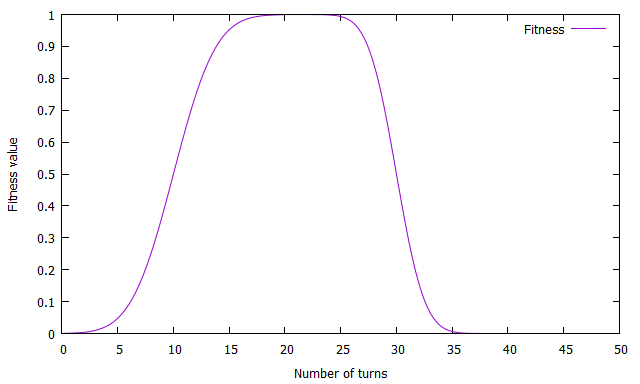
\includegraphics[width=0.75\textwidth]{img/game-length-fitness.png}
	\caption{Fitness values for games of a given length, determined by two combined cumulative normal distribution functions.}
	\label{fig:game-length}	
\end{figure}

\begin{figure}
	\centering
	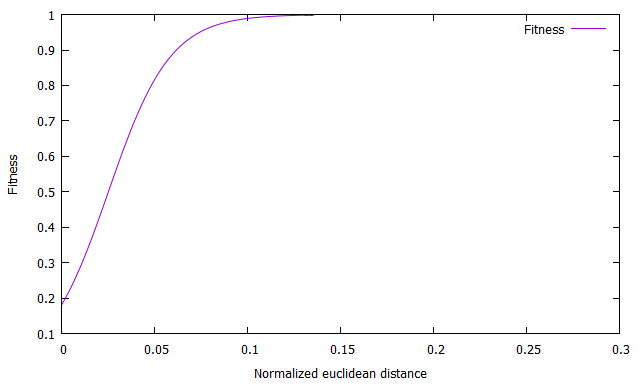
\includegraphics[width=0.75\textwidth]{img/team-distance.png}
	\caption{Fitness values for normalized euclidean distance between the two teams. Showing only the section where distance is less than $30\%$.}
	\label{fig:team-distance}	
\end{figure}


\begin{figure}
	\centering
	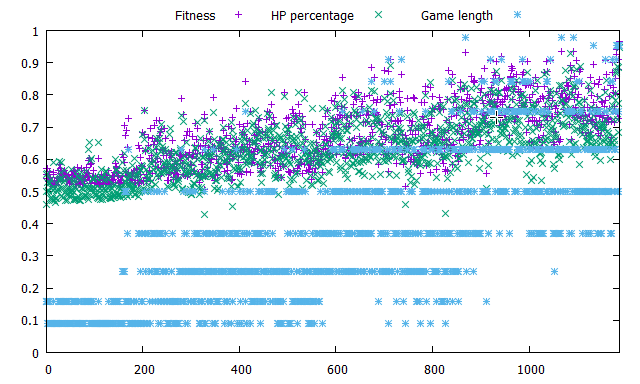
\includegraphics[width=0.75\textwidth]{img/converging-es.png}
	\caption{An example of a how the combined fitness function converges over rougly 1200 iterations. Green dots represent the \emph{Balance} fitness measuring HP percentage left at the end of the game, blue dots represent game length, and purple is the combined fitness. We're not showing team difference data points as in this plot.}
	\label{fig:converging-es}	
\end{figure}

\section{Remarks}

During the experiment we encountered multiple ways ES tried to exploit the
game mechanics to maximize the balance fitness function in ways that were
undesirable. One example being when the resulting games end up being short
as the algorithm generates mages with lots of AOE abilities that cover the
whole map in the first turn, resulting in immediate death of all characters.

We balance this by introducing an additional fitness function for game length
in the form of a cumulative normal distribution with mean around $10$ turns.

Lastly, the team difference is measured as an euclidean distance between the DNA
vectors of each team. Again, we use a cumulative normal distribution to put a lower
bound on the team difference.
